% answers.tex —— 2007 年·普通高等学校招生考试·重庆卷·文科 · 参考答案与详细解析片段
% 由 tools/generate_projects.py 依来源总账自 2007/2007_数学真题_重庆文_试题.md + 2007/2007_数学真题_重庆文_解析正文.md + 2007/2007_数学真题_重庆文_答案要点.md 生成，勿手改（改源 MD 后重跑）


\begin{gktip}
固定候选 PDF 仅含题面，无答案、解析和评分标准，原卷亦未标注分值；以下为非官方编者独立推导，官方答案字段为空。来源发布者、出版者、版次与官方身份均未核。
\end{gktip}

\begin{answer}
\gksolhead{1}{}

\textbf{题目}：

在等比数列 $\{a_n\}$ 中，$a_2=8$，$a_1=64$，则公比 $q$ 为（　）

（A）$2$

（B）$3$

（C）$4$

（D）$8$

\Needspace{4\baselineskip}
\textbf{解析}

\Needspace{5\baselineskip}
等比数列中 $a_2=a_1q$，故

\nopagebreak[4]
\[q=\frac{a_2}{a_1}=\frac8{64}=\frac18.\]

四个选项只有 (D) 与 $8$ 相关，按命题意图（$a_1$ 与 $a_2$ 的数值印反，正确应为 $a_1=8$，$a_2=64$）取 $q=8$。

【源疑点：原页印「$a_2=8$，$a_1=64$」，据此算得 $q=\frac18$，与四个选项（$2$，$3$，$4$，$8$）均不相符；按选项反推应为 $a_1=8$，$a_2=64$，此时 $q=8$，本库取 (D)。】

\gkanswer{答案：D。}

\end{answer}
\begin{answer}
\gksolhead{2}{}

\textbf{题目}：

设全集 $U=\{a,b,c,d\}$，$A=\{a,c\}$，$B=\{b\}$，则 $A\cap(\complement_UB)=$（　）

（A）$\varnothing$

（B）$\{a\}$

（C）$\{c\}$

（D）$\{a,c\}$

\Needspace{4\baselineskip}
\textbf{解析}

\Needspace{5\baselineskip}
$\complement_UB=\{a,c,d\}$，故

\nopagebreak[4]
\[A\cap(\complement_UB)=\{a,c\}\cap\{a,c,d\}=\{a,c\}.\]

\gkanswer{答案：D。}

\end{answer}
\begin{answer}
\gksolhead{3}{}

\textbf{题目}：

垂直于同一平面的两条直线（　）

（A）平行

（B）垂直

（C）相交

（D）异面

\Needspace{4\baselineskip}
\textbf{解析}

垂直于同一平面的两条直线方向都与该平面的法向量平行，故互相平行。

\gkanswer{答案：A。}

\end{answer}
\begin{answer}
\gksolhead{4}{}

\textbf{题目}：

$(2x-1)^6$ 展开式中 $x^2$ 的系数为（　）

（A）$15$

（B）$60$

（C）$120$

（D）$240$

\Needspace{4\baselineskip}
\textbf{解析}

\Needspace{5\baselineskip}
含 $x^2$ 的项为

\nopagebreak[4]
\[\mathrm C_6^2(2x)^2(-1)^4=15\times4x^2=60x^2,\]

故系数为 $60$。

\gkanswer{答案：B。}

\end{answer}
\begin{answer}
\gksolhead{5}{}

\textbf{题目}：

“$-1<x<1$”是“$x^2<1$”的（　）

（A）充分必要条件

（B）充分但不必要条件

（C）必要但不充分条件

（D）既不充分也不必要条件

\Needspace{4\baselineskip}
\textbf{解析}

\Needspace{5\baselineskip}
计算如下：

\nopagebreak[4]
\[x^2<1\ \Longleftrightarrow\ -1<x<1,\]

两个条件互为充要条件。

\gkanswer{答案：A。}

\end{answer}
\begin{answer}
\gksolhead{6}{}

\textbf{题目}：

下列各式中，值为 $\dfrac{\sqrt3}{2}$ 的是（　）

（A）$2\sin15^\circ\cos15^\circ$

（B）$\cos^215^\circ-\sin^215^\circ$

（C）$2\sin^215^\circ-1$

（D）$\sin^215^\circ+\cos^215^\circ$

\Needspace{4\baselineskip}
\textbf{解析}

\Needspace{5\baselineskip}
逐项用倍角公式：

\nopagebreak[4]
\[2\sin15^\circ\cos15^\circ=\sin30^\circ=\frac12,\]

\nopagebreak[4]
\[\cos^215^\circ-\sin^215^\circ=\cos30^\circ=\frac{\sqrt3}2,\]

\nopagebreak[4]
\[2\sin^215^\circ-1=-\cos30^\circ=-\frac{\sqrt3}2,\qquad \sin^215^\circ+\cos^215^\circ=1.\]

\gkanswer{答案：B。}

\end{answer}
\begin{answer}
\gksolhead{7}{}

\textbf{题目}：

从 $5$ 张 $100$ 元，$3$ 张 $200$ 元，$2$ 张 $300$ 元的奥运预赛门票中任取 $3$ 张，则所取 $3$ 张中至少有 $2$ 张价格相同的概率为（　）

（A）$\dfrac14$

（B）$\dfrac{79}{120}$

（C）$\dfrac34$

（D）$\dfrac{23}{24}$

\Needspace{4\baselineskip}
\textbf{解析}

\Needspace{5\baselineskip}
任取 $3$ 张共 $\mathrm C_{10}^3=120$ 种。三张价格互不相同需从三类各取一张，共

\nopagebreak[4]
\[5\times3\times2=30\]

\Needspace{5\baselineskip}
种，故至少两张同价的有 $120-30=90$ 种，概率

\nopagebreak[4]
\[P=\frac{90}{120}=\frac34.\]

\gkanswer{答案：C。}

\end{answer}
\begin{answer}
\gksolhead{8}{}

\textbf{题目}：

若直线 $y=kx+1$ 与圆 $x^2+y^2=1$ 相交于 $P$，$Q$ 两点，且 $\angle POQ=120^\circ$（其中 $O$ 为原点），则 $k$ 的值为（　）

（A）$-\sqrt3$ 或 $\sqrt3$

（B）$\sqrt3$

（C）$-\sqrt2$ 或 $\sqrt2$

（D）$\sqrt2$

\Needspace{4\baselineskip}
\textbf{解析}

\Needspace{5\baselineskip}
圆心到直线 $kx-y+1=0$ 的距离

\nopagebreak[4]
\[d=\frac1{\sqrt{k^2+1}}.\]

\Needspace{5\baselineskip}
弦 $PQ$ 对应的圆心角为 $120^\circ$，故弦心距

\nopagebreak[4]
\[d=\cos60^\circ=\frac12,\]

即 $\dfrac1{\sqrt{k^2+1}}=\dfrac12$，得 $k^2=3$，$k=\pm\sqrt3$。

\gkanswer{答案：A。}

\end{answer}
\begin{answer}
\gksolhead{9}{}

\textbf{题目}：

已知向量 $\overrightarrow{OA}=(4,6)$，$\overrightarrow{OB}=(3,5)$，且 $\overrightarrow{OC}\perp\overrightarrow{OA}$，$\overrightarrow{AC}\parallel\overrightarrow{OB}$，则向量 $\overrightarrow{OC}=$（　）

（A）$\left(-\dfrac37,\dfrac27\right)$

（B）$\left(-\dfrac27,\dfrac4{21}\right)$

（C）$\left(\dfrac37,-\dfrac27\right)$

（D）$\left(\dfrac27,-\dfrac4{21}\right)$

\Needspace{4\baselineskip}
\textbf{解析}

\Needspace{5\baselineskip}
设 $\overrightarrow{OC}=(x,y)$。由 $\overrightarrow{OC}\perp\overrightarrow{OA}$：

\nopagebreak[4]
\[4x+6y=0\ \Rightarrow\ y=-\frac23x.\]

\Needspace{5\baselineskip}
又 $\overrightarrow{AC}=(x-4,y-6)\parallel\overrightarrow{OB}=(3,5)$，故

\nopagebreak[4]
\[5(x-4)=3(y-6)\ \Rightarrow\ 5x-3y=2.\]

\Needspace{5\baselineskip}
代入 $y=-\dfrac23x$ 得 $5x+2x=2$，$x=\dfrac27$，$y=-\dfrac4{21}$，即

\nopagebreak[4]
\[\overrightarrow{OC}=\left(\frac27,-\frac4{21}\right).\]

\gkanswer{答案：D。}

\end{answer}
\begin{answer}
\gksolhead{10}{}

\textbf{题目}：

设 $P(3,1)$ 为二次函数 $f(x)=ax^2-2ax+b$（$x\geqslant1$）的图象与其反函数 $y=f^{-1}(x)$ 的图象的一个交点，则（　）

（A）$a=\dfrac12$，$b=\dfrac52$

（B）$a=\dfrac12$，$b=-\dfrac52$

（C）$a=-\dfrac12$，$b=\dfrac52$

（D）$a=-\dfrac12$，$b=-\dfrac52$

\Needspace{4\baselineskip}
\textbf{解析}

\Needspace{5\baselineskip}
$P(3,1)$ 在 $y=f(x)$ 上：

\nopagebreak[4]
\[9a-6a+b=1\ \Rightarrow\ 3a+b=1.\]

\Needspace{5\baselineskip}
$P$ 又在 $y=f^{-1}(x)$ 上，等价于 $(1,3)$ 在 $y=f(x)$ 上：

\nopagebreak[4]
\[a-2a+b=3\ \Rightarrow\ b-a=3.\]

\Needspace{5\baselineskip}
联立得 $b=1-3a$ 且 $b=a+3$，故

\nopagebreak[4]
\[1-3a=a+3\ \Rightarrow\ a=-\frac12,\qquad b=\frac52.\]

\gkanswer{答案：C。}

\end{answer}
\begin{answer}
\gksolhead{11}{}

\textbf{题目}：

设 $\sqrt3b$ 是 $1-a$ 和 $1+a$ 的等比中项，则 $a+3b$ 的最大值为（　）

（A）$1$

（B）$2$

（C）$3$

（D）$4$

\Needspace{4\baselineskip}
\textbf{解析}

\Needspace{5\baselineskip}
$\sqrt3b$ 是 $1-a$ 与 $1+a$ 的等比中项，故

\nopagebreak[4]
\[3b^2=(1-a)(1+a)=1-a^2,\]

\Needspace{5\baselineskip}
即 $b=\sqrt{\dfrac{1-a^2}3}$（$|a|\leqslant1$，$b\geqslant0$）。于是

\nopagebreak[4]
\[a+3b=a+\sqrt3\sqrt{1-a^2}.\]

\Needspace{5\baselineskip}
令 $a=\cos t$，$t\in[0,\pi]$，则 $\sqrt{1-a^2}=\sin t$，

\nopagebreak[4]
\[a+3b=\cos t+\sqrt3\sin t=2\sin\left(t+\frac{\pi}6\right)\leqslant2,\]

等号当 $t=\dfrac{\pi}3$（即 $a=\dfrac12$，$b=\dfrac12$）时成立。

\gkanswer{答案：B。}

\end{answer}
\begin{answer}
\gksolhead{12}{}

\textbf{题目}：

已知以 $F_1(-2,0)$，$F_2(2,0)$ 为焦点的椭圆与直线 $x+\sqrt3y+4=0$ 有且仅有一个交点，则椭圆的长轴长为（　）

（A）$3\sqrt2$

（B）$2\sqrt6$

（C）$2\sqrt7$

（D）$4\sqrt2$

\Needspace{4\baselineskip}
\textbf{解析}

\Needspace{5\baselineskip}
设椭圆为 $\dfrac{x^2}{a^2}+\dfrac{y^2}{b^2}=1$，$c=2$，$b^2=a^2-4$。直线 $x+\sqrt3y+4=0$ 与椭圆相切 $\Leftrightarrow$

\nopagebreak[4]
\[a^2\cdot1^2+b^2\cdot(\sqrt3)^2=4^2,\]

\Needspace{5\baselineskip}
即

\nopagebreak[4]
\[a^2+3(a^2-4)=16\ \Rightarrow\ 4a^2=28\ \Rightarrow\ a=\sqrt7.\]

长轴长 $2a=2\sqrt7$。

\gkanswer{答案：C。}

\end{answer}
\begin{answer}
\gksolhead{13}{}

\textbf{题目}：

在 $\triangle ABC$ 中，$AB=1$，$BC=2$，$B=60^\circ$，则 $AC=$\gkblank{}。

\Needspace{4\baselineskip}
\textbf{解析}

\Needspace{5\baselineskip}
由余弦定理

\nopagebreak[4]
\[AC^2=AB^2+BC^2-2\cdot AB\cdot BC\cos B=1+4-2\times1\times2\times\frac12=3,\]

故 $AC=\sqrt3$。

\gkanswer{答案：$\sqrt3$。}

\end{answer}
\begin{answer}
\gksolhead{14}{}

\textbf{题目}：

已知 $\begin{cases}2x+3y\leqslant6,\\ x-y\geqslant0,\\ y\geqslant0,\end{cases}$ 则 $z=3x-y$ 的最大值为\gkblank{}。

\Needspace{4\baselineskip}
\textbf{解析}

\Needspace{5\baselineskip}
可行域顶点为 $(0,0)$，$(3,0)$ 与（两直线交点）$\left(\dfrac65,\dfrac65\right)$。计算

\nopagebreak[4]
\[z=3x-y:\quad 0,\quad 9,\quad \frac{12}5,\]

故最大值为 $9$。

\gkanswer{答案：$9$。}

\end{answer}
\begin{answer}
\gksolhead{15}{}

\textbf{题目}：

要排出某班一天中语文、数学、政治、英语、体育、艺术 $6$ 门课各一节的课程表，要求数学课排在前 $3$ 节，英语课不排在第 $6$ 节，则不同的排法种数为\gkblank{}。（以数字作答）

\Needspace{4\baselineskip}
\textbf{解析}

\Needspace{5\baselineskip}
数学排在前 $3$ 节：$3\times5!=360$ 种。其中英语排第 $6$ 节的有 $3\times4!=72$ 种（数学占前 $3$ 节之一，其余 $4$ 门任排）。故

\nopagebreak[4]
\[360-72=288.\]

\gkanswer{答案：$288$。}

\end{answer}
\begin{answer}
\gksolhead{16}{}

\textbf{题目}：

函数 $f(x)=\sqrt{x^2-2x}+2\sqrt{x^2-5x+4}$ 的最小值为\gkblank{}。

\Needspace{4\baselineskip}
\textbf{解析}

\Needspace{5\baselineskip}
定义域由 $x^2-2x\geqslant0$ 与 $x^2-5x+4\geqslant0$ 共同给出：

\nopagebreak[4]
\[x\leqslant0\quad\text{\text{或}}\quad x\geqslant4.\]

\Needspace{5\baselineskip}
在 $x\leqslant0$ 上两个根式都随 $x$ 增大而减小，故最小值在 $x=0$ 取到，为

\nopagebreak[4]
\[f(0)=0+2\sqrt4=4.\]

\Needspace{5\baselineskip}
在 $x\geqslant4$ 上两个根式都递增，最小值在 $x=4$ 取到：

\nopagebreak[4]
\[f(4)=\sqrt{16-8}+0=2\sqrt2<4.\]

故最小值为 $2\sqrt2$。

\gkanswer{答案：$2\sqrt2$。}

\end{answer}
\begin{answer}
\gksolhead{17}{}

\textbf{题目}：

设甲、乙两人每次射击命中目标的概率分别为 $\dfrac34$ 和 $\dfrac45$，且各次射击相互独立。

（1）若甲、乙各射击一次，求甲命中但乙未命中目标的概率；

（2）若甲、乙各射击两次，求两人命中目标的次数相等的概率。

\Needspace{4\baselineskip}
\textbf{解析}

记甲、乙命中概率 $p_1=\dfrac34$，$p_2=\dfrac45$，未命中概率 $q_1=\dfrac14$，$q_2=\dfrac15$。

\Needspace{5\baselineskip}
（1）甲中乙不中：

\nopagebreak[4]
\[P=p_1q_2=\frac34\times\frac15=\frac3{20}.\]

\Needspace{5\baselineskip}
（2）各射两次，命中次数 $X\sim B(2,p_1)$，$Y\sim B(2,p_2)$，独立。逐项计算：

\nopagebreak[4]
\[P(X=2)=\frac9{16},\quad P(X=1)=\frac38,\quad P(X=0)=\frac1{16},\]

\nopagebreak[4]
\[P(Y=2)=\frac{16}{25},\quad P(Y=1)=\frac8{25},\quad P(Y=0)=\frac1{25}.\]

\Needspace{5\baselineskip}
故

\nopagebreak[4]
\[P(X=Y)=\frac9{16}\cdot\frac{16}{25}+\frac38\cdot\frac8{25}+\frac1{16}\cdot\frac1{25}
=\frac9{25}+\frac3{25}+\frac1{400}=\frac{193}{400}.\]

\gkanswer{答案：（1）$\dfrac3{20}$；（2）$\dfrac{193}{400}$。}

\end{answer}
\begin{answer}
\gksolhead{18}{}

\textbf{题目}：

已知函数 $f(x)=\dfrac{1+\sqrt2\cos\left(2x-\dfrac{\pi}{4}\right)}{\sin\left(x+\dfrac{\pi}{2}\right)}$。

（1）求 $f(x)$ 的定义域；

（2）若角 $\alpha$ 在第一象限且 $\cos\alpha=\dfrac35$，求 $f(\alpha)$。

\Needspace{4\baselineskip}
\textbf{解析}

\Needspace{5\baselineskip}
（1）$\sin\left(x+\dfrac{\pi}2\right)=\cos x$，分母不为零，故

\nopagebreak[4]
\[\cos x\neq0\ \Rightarrow\ x\neq\frac{\pi}2+k\pi\quad(k\in\mathbf Z).\]

\Needspace{5\baselineskip}
（2）$\alpha$ 在第一象限且 $\cos\alpha=\dfrac35$，故 $\sin\alpha=\dfrac45$，

\nopagebreak[4]
\[\cos2\alpha=2\cos^2\alpha-1=-\frac7{25},\qquad \sin2\alpha=2\sin\alpha\cos\alpha=\frac{24}{25}.\]

\Needspace{5\baselineskip}
分子

\nopagebreak[4]
\[1+\sqrt2\cos\left(2\alpha-\frac{\pi}4\right)=1+\sqrt2\left(\frac{\sqrt2}2\cos2\alpha+\frac{\sqrt2}2\sin2\alpha\right)=1+\cos2\alpha+\sin2\alpha,\]

\Needspace{5\baselineskip}
即

\nopagebreak[4]
\[1-\frac7{25}+\frac{24}{25}=\frac{42}{25}.\]

\Needspace{5\baselineskip}
分母 $\cos\alpha=\dfrac35$，故

\nopagebreak[4]
\[f(\alpha)=\frac{42/25}{3/5}=\frac{42}{25}\times\frac53=\frac{14}5.\]

\gkanswer{答案：（1）$\left\{x\ \middle|\ x\neq\dfrac{\pi}2+k\pi,\ k\in\mathbf Z\right\}$；（2）$\dfrac{14}5$。}

\end{answer}
\begin{answer}
\gksolhead{19}{}

\textbf{题目}：

如图，在直三棱柱 $ABC-A_1B_1C_1$ 中，$\angle ABC=90^\circ$，$AB=1$，$BC=\dfrac32$，$AA_1=2$；点 $D$ 在棱 $BB_1$ 上，$BD=\dfrac13BB_1$；$B_1E\perp A_1D$，垂足为 $E$。求：

（1）异面直线 $A_1D$ 与 $B_1C_1$ 的距离；

（2）四棱锥 $C-ABDE$ 的体积。
\nopagebreak[4]
\begin{center}% 2007 年重庆卷文科第 19 题：直三棱柱 ABC-A1B1C1，∠ABC=90°，AB=1，BC=3/2，AA1=2；
%   D 在 BB1 上且 BD=BB1/3，B1E⊥A1D 于 E。图中 E 位于 A1D 上、B1 的左下方。
% 来源 PDF：gaokaomath-src/普通高考/2007/2007重庆文.pdf
% SHA-256：a647b60227db10d70c5c3fbe72b6ffe2c8a0667b233695e55bb4f5a7cef633a6
% 原页：2007重庆文.pdf 第 1 页（A3 三栏）第 3 栏，书页码 357。
% 重绘依据：按原页 A1、C1、B1、E、D、A、B、C 的相对位置与虚实线重绘；
%   斜投影的深度偏移取 0.55，使 D（BB1 的三分之一处）与底面对角线 AC 在图上分开。
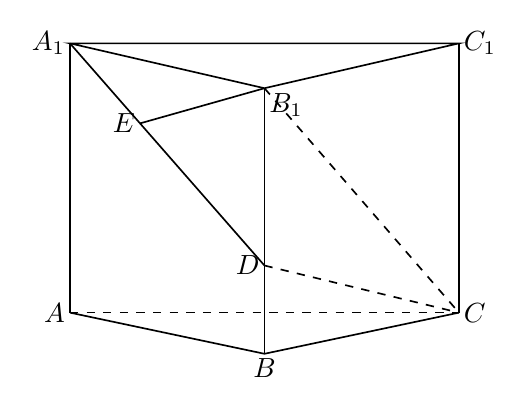
\begin{tikzpicture}[scale=0.95, semithick,
  every node/.style={inner sep=1.5pt}]

  \coordinate (A)  at (0.0,0.55);
  \coordinate (B)  at (2.60,0.00);
  \coordinate (C)  at (5.20,0.55);
  \coordinate (A1) at (0.0,4.15);
  \coordinate (B1) at (2.60,3.55);
  \coordinate (C1) at (5.20,4.15);
  \coordinate (D)  at (2.60,1.18);
  \coordinate (E)  at (0.936,3.08);

  % 底面
  \draw (A) -- (B) -- (C);
  \draw[dashed] (A) -- (C);
  % 侧棱
  \draw (A) -- (A1);
  \draw (B) -- (B1);
  \draw (C) -- (C1);
  % 上底面
  \draw (A1) -- (B1) -- (C1) -- cycle;

  % 题设连线
  \draw (A1) -- (D);
  \draw (B1) -- (E);
  \draw[dashed] (B1) -- (C);
  \draw[dashed] (D) -- (C);

  \node[left] at (A) {$A$};
  \node[below] at (B) {$B$};
  \node[right] at (C) {$C$};
  \node[left] at (A1) {$A_1$};
  \node[below right] at (B1) {$B_1$};
  \node[right] at (C1) {$C_1$};
  \node[left] at (D) {$D$};
  \node[left] at (E) {$E$};
\end{tikzpicture}
\end{center}
\nopagebreak[4]
\Needspace{4\baselineskip}
\textbf{解析}

\Needspace{5\baselineskip}
以 $B$ 为原点，$BA$，$BC$，$BB_1$ 为 $x$，$y$，$z$ 轴：

\nopagebreak[4]
\[B(0,0,0),\ A(1,0,0),\ C\left(0,\frac32,0\right),\ A_1(1,0,2),\ B_1(0,0,2),\ C_1\left(0,\frac32,2\right),\]

\nopagebreak[4]
\[D\left(0,0,\frac23\right).\]

\Needspace{5\baselineskip}
（1）$B_1C_1$ 的方向为 $(0,1,0)$，且 $A_1D$ 在平面 $y=0$ 内。把两直线投影到 $xz$ 平面：$B_1C_1$ 投影为点 $(0,2)$，$A_1D$ 投影为过 $(1,2)$、$\left(0,\frac23\right)$ 的直线，方向 $(-1,-\frac43)$。点 $(0,2)$ 到该直线的距离

\nopagebreak[4]
\[d=\frac{\left|(-1,0)\times\left(-1,-\frac43\right)\right|}{\sqrt{1+\frac{16}9}}
=\frac{\frac43}{\frac53}=\frac45.\]

\Needspace{5\baselineskip}
（2）$E$ 是 $B_1$ 到 $A_1D$ 的垂足：

\nopagebreak[4]
\[\overrightarrow{A_1D}=\left(-1,0,-\frac43\right),\qquad \overrightarrow{A_1B_1}=(-1,0,0),\]

\nopagebreak[4]
\[t=\frac{\overrightarrow{A_1B_1}\cdot\overrightarrow{A_1D}}{\left|\overrightarrow{A_1D}\right|^2}
=\frac{1}{\frac{25}9}=\frac9{25},\]

\Needspace{5\baselineskip}
故

\nopagebreak[4]
\[E=A_1+\frac9{25}\overrightarrow{A_1D}=\left(\frac{16}{25},0,\frac{38}{25}\right).\]

\Needspace{5\baselineskip}
四边形 $ABDE$ 在平面 $y=0$ 内，用 $A$，$B$，$D$，$E$ 的 $xz$ 坐标算面积：

\nopagebreak[4]
\[S_{\triangle ABD}=\frac12\times1\times\frac23=\frac13,\]

\nopagebreak[4]
\[S_{\triangle ADE}=\frac12\left|(-1)\left(\frac{38}{25}\right)-\left(\frac23\right)\left(-\frac9{25}\right)\right|
=\frac12\cdot\frac{32}{25}=\frac{16}{25},\]

\nopagebreak[4]
\[S_{ABDE}=\frac13+\frac{16}{25}=\frac{73}{75}.\]

\Needspace{5\baselineskip}
点 $C$ 到平面 $y=0$ 的距离为 $\dfrac32$，故

\nopagebreak[4]
\[V=\frac13\cdot\frac{73}{75}\cdot\frac32=\frac{73}{150}.\]

\gkanswer{答案：（1）$\dfrac45$；（2）$\dfrac{73}{150}$。}

\end{answer}
\begin{answer}
\gksolhead{20}{}

\textbf{题目}：

用长为 $18\ \mathrm m$ 的钢条围成一个长方体形状的框架，要求长方体的长与宽之比为 $2:1$，问该长方体的长、宽、高各为多少时，其体积最大？最大体积是多少？

\Needspace{4\baselineskip}
\textbf{解析}

\Needspace{5\baselineskip}
设宽为 $w$，则长为 $2w$，高为 $h$。长方体框架共 $4$ 条长、$4$ 条宽、$4$ 条高：

\nopagebreak[4]
\[4(2w+w+h)=18\ \Rightarrow\ 3w+h=\frac92\ \Rightarrow\ h=\frac92-3w.\]

\Needspace{5\baselineskip}
体积

\nopagebreak[4]
\[V=2w\cdot w\cdot h=9w^2-6w^3,\qquad 0<w<\frac32.\]

\Needspace{5\baselineskip}
求导：

\nopagebreak[4]
\[V'=18w-18w^2=18w(1-w).\]

\Needspace{5\baselineskip}
$0<w<1$ 时 $V'>0$，$1<w<\dfrac32$ 时 $V'<0$，故 $w=1$ 时体积最大：

\nopagebreak[4]
\[V_{\max}=9-6=3.\]

此时长 $2$，宽 $1$，高 $h=\dfrac92-3=\dfrac32$，即高为 $\dfrac32\ \mathrm m$。

\gkanswer{答案：长 $2\ \mathrm m$、宽 $1\ \mathrm m$、高 $\dfrac32\ \mathrm m$，最大体积 $3\ \mathrm{m^3}$。}

\end{answer}
\begin{answer}
\gksolhead{21}{}

\textbf{题目}：

如图，倾斜角为 $\alpha$ 的直线经过抛物线 $y^2=8x$ 的焦点 $F$，且与抛物线交于 $A$、$B$ 两点。

（1）求抛物线的焦点 $F$ 的坐标及准线 $l$ 方程；

（2）若 $\alpha$ 为锐角，作线段 $AB$ 的垂直平分线 $m$ 交 $x$ 轴于点 $P$，证明 $|FP|-|FP|\cos2\alpha$ 为定值，并求此定值。
\nopagebreak[4]
\begin{center}% 2007 年重庆卷文科第 21 题：抛物线 y^2=8x、焦点 F、准线 l 与过 F 的直线交于 A、B；
%   弦 AB 的垂直平分线 m 交 x 轴于 P，倾斜角 α 标在直线与 x 轴之间。
% 来源 PDF：gaokaomath-src/普通高考/2007/2007重庆文.pdf
% SHA-256：a647b60227db10d70c5c3fbe72b6ffe2c8a0667b233695e55bb4f5a7cef633a6
% 原页：2007重庆文.pdf 第 2 页（A3 三栏）第 2 栏，书页码 358。
% 重绘依据：按 α=60° 作图（A 在上、B 在下、P 在焦点右侧）；m 取过弦中点 M(10/3,2√3)、
%   斜率 −1/√3 的直线，与 x 轴的交点即 P(22/3,0)，与原页位置关系一致。
\begin{tikzpicture}[x=0.78cm, y=0.52cm, semithick,
  every node/.style={inner sep=1.5pt}]

  % 坐标轴
  \draw[->,>=stealth] (-2.8,0) -- (8.6,0) node[right] {$x$};
  \draw[->,>=stealth] (0,-7.6) -- (0,8.2) node[above] {$y$};
  \node[below left] at (0,0) {$O$};

  % 准线 l：x=-2
  \draw (-2,-7.2) -- (-2,7.6) node[above] {$l$};

  % 抛物线 y^2=8x
  \draw[domain=-7.2:7.2,samples=160,line width=1pt] plot ({\x*\x/8},{\x});

  % 过 F 的直线（α=60°），交抛物线于 A、B
  \coordinate (F) at (2,0);
  \coordinate (A) at (6,6.928);
  \coordinate (B) at (0.667,-2.309);
  \draw (B) -- (A);

  % 弦 AB 的垂直平分线 m（过中点 M，斜率 -1/√3），交 x 轴于 P
  \coordinate (P) at (7.333,0);
  \draw (1.2,3.539) -- (8.3,-0.559);
  \node[above left] at (1.2,3.539) {$m$};

  % 角 α
  \draw (2.9,0) arc[start angle=0,end angle=60,radius=0.9];
  \node at (3.35,0.95) {$\alpha$};

  \fill (F) circle (1.3pt);
  \fill (P) circle (1.3pt);
  \node[below right=2pt] at (F) {$F$};
  \node[below=3pt] at (P) {$P$};
  \node[above left] at (A) {$A$};
  \node[below left] at (B) {$B$};
\end{tikzpicture}
\end{center}
\nopagebreak[4]
\Needspace{4\baselineskip}
\textbf{解析}

（1）$y^2=8x=2px$ 中 $2p=8$，$p=4$，故焦点 $F\left(\dfrac p2,0\right)=(2,0)$，准线 $x=-\dfrac p2=-2$。

\Needspace{5\baselineskip}
（2）设直线 $AB$ 的斜率为 $t=\tan\alpha$（$\alpha$ 为锐角，$t>0$），方程为 $y=t(x-2)$。代入 $y^2=8x$：

\nopagebreak[4]
\[t^2(x-2)^2=8x,\]

\nopagebreak[4]
\[t^2x^2-(4t^2+8)x+4t^2=0.\]

\Needspace{5\baselineskip}
设 $A(x_1,y_1)$，$B(x_2,y_2)$，则

\nopagebreak[4]
\[x_1+x_2=\frac{4t^2+8}{t^2}=4+\frac8{t^2}.\]

\Needspace{5\baselineskip}
中点 $M$ 的坐标

\nopagebreak[4]
\[x_M=2+\frac4{t^2},\qquad y_M=t(x_M-2)=\frac4t.\]

\Needspace{5\baselineskip}
垂直平分线 $m$ 过 $M$、斜率为 $-\dfrac1t$，令 $y=0$ 得

\nopagebreak[4]
\[x_P=x_M+t\,y_M=2+\frac4{t^2}+4=6+\frac4{t^2}.\]

\Needspace{5\baselineskip}
于是

\nopagebreak[4]
\[|FP|=x_P-2=4+\frac4{t^2}=4\left(1+\frac1{\tan^2\alpha}\right)=\frac4{\sin^2\alpha}.\]

\Needspace{5\baselineskip}
又 $1-\cos2\alpha=2\sin^2\alpha$，故

\nopagebreak[4]
\[|FP|-|FP|\cos2\alpha=|FP|(1-\cos2\alpha)=\frac4{\sin^2\alpha}\cdot2\sin^2\alpha=8,\]

为定值。

\gkanswer{答案：（1）$F(2,0)$，$l:x=-2$；（2）定值 $8$。}

\end{answer}
\begin{answer}
\gksolhead{22}{}

\textbf{题目}：

已知各项均为正数的数列 $\{a_n\}$ 的前 $n$ 项和 $S_n$ 满足 $S_1>1$，且 $6S_n=(a_n+1)(a_n+2)$，$n\in\mathbf N_+$。

（1）求 $\{a_n\}$ 的通项公式；

（2）设数列 $\{b_n\}$ 满足 $a_n(2^{b_n}-1)=1$，并记 $T_n$ 为 $\{b_n\}$ 的前 $n$ 项和，求证：$3T_n+1>\log_2(a_n+3)$，$n\in\mathbf N_+$。

\Needspace{4\baselineskip}
\textbf{解析}

\Needspace{5\baselineskip}
（1）$n=1$ 时 $6S_1=6a_1=(a_1+1)(a_1+2)$，即

\nopagebreak[4]
\[a_1^2-3a_1+2=0,\]

故 $a_1=1$ 或 $a_1=2$；由 $S_1=a_1>1$ 得 $a_1=2$。

\Needspace{5\baselineskip}
$n\geqslant2$ 时，与 $6S_{n-1}=(a_{n-1}+1)(a_{n-1}+2)$ 相减：

\nopagebreak[4]
\[6a_n=a_n^2-a_{n-1}^2+3a_n-3a_{n-1},\]

\Needspace{5\baselineskip}
整理得

\nopagebreak[4]
\[(a_n+a_{n-1})(a_n-a_{n-1}-3)=0.\]

\Needspace{5\baselineskip}
各项为正，故 $a_n-a_{n-1}=3$，即 $\{a_n\}$ 是首项 $2$、公差 $3$ 的等差数列：

\nopagebreak[4]
\[a_n=3n-1.\]

\Needspace{5\baselineskip}
（2）由 $a_n(2^{b_n}-1)=1$ 得

\nopagebreak[4]
\[2^{b_n}=1+\frac1{a_n}=\frac{a_n+1}{a_n}=\frac{3n}{3n-1},\]

\Needspace{5\baselineskip}
故

\nopagebreak[4]
\[b_n=\log_2\frac{3n}{3n-1},\]

\nopagebreak[4]
\[T_n=\sum_{k=1}^n\log_2\frac{3k}{3k-1}=\log_2\prod_{k=1}^n\frac{3k}{3k-1}.\]

\Needspace{5\baselineskip}
记 $P_n=\prod_{k=1}^{n}\dfrac{3k}{3k-1}$。对每个正整数 $k$，

\nopagebreak[4]
\[(3k)^3-(3k+2)(3k-1)^2=27k^3-(27k^3-9k+2)=9k-2>0,\]

\Needspace{5\baselineskip}
故

\nopagebreak[4]
\[\left(\frac{3k}{3k-1}\right)^3>\frac{3k+2}{3k-1}.\]

\Needspace{5\baselineskip}
累乘得

\nopagebreak[4]
\[P_n^3>\prod_{k=1}^n\frac{3k+2}{3k-1}=\frac{5\cdot8\cdots(3n+2)}{2\cdot5\cdots(3n-1)}=\frac{3n+2}2.\]

\Needspace{5\baselineskip}
于是

\nopagebreak[4]
\[2P_n^3>3n+2,\]

\Needspace{5\baselineskip}
两边取以 $2$ 为底的对数：

\nopagebreak[4]
\[\log_2(2P_n^3)>\log_2(3n+2),\]

\Needspace{5\baselineskip}
即

\nopagebreak[4]
\[3T_n+1>\log_2(3n+2)=\log_2(a_n+3).\]

故所证不等式成立。

\gkanswer{答案：（1）$a_n=3n-1$；（2）证明见解析。}

\end{answer}